% Created 2024-06-11 Τρι 13:30
% Intended LaTeX compiler: pdflatex
\documentclass[11pt]{article}
\usepackage[utf8]{inputenc}
\usepackage[T1]{fontenc}
\usepackage{graphicx}
\usepackage{longtable}
\usepackage{wrapfig}
\usepackage{rotating}
\usepackage[normalem]{ulem}
\usepackage{amsmath}
\usepackage{amssymb}
\usepackage{capt-of}
\usepackage{hyperref}
\usepackage{booktabs}
\usepackage{import}
\usepackage[LGR, T1]{fontenc}
\usepackage[greek, english, american]{babel}
\usepackage{alphabeta}
\usepackage{esint}
\usepackage{mathtools}
\usepackage{esdiff}
\usepackage{makeidx}
\usepackage[acronym]{glossaries}
\usepackage{newfloat}
\usepackage{minted}
\usepackage[a4paper, margin=3cm]{geometry}
\usepackage{chemfig}
\usepackage{svg}
\author{Vidianos Giannitsis}
\date{\today}
\title{Αναλύσεις της τροφοδοσίας της αναερόβιας χώνευσης}
\hypersetup{
 pdfauthor={Vidianos Giannitsis},
 pdftitle={Αναλύσεις της τροφοδοσίας της αναερόβιας χώνευσης},
 pdfkeywords={},
 pdfsubject={},
 pdfcreator={Emacs 29.3 (Org mode 9.6.15)}, 
 pdflang={English}}
\makeatletter
\newcommand{\citeprocitem}[2]{\hyper@linkstart{cite}{citeproc_bib_item_#1}#2\hyper@linkend}
\makeatother

\usepackage[notquote]{hanging}
\begin{document}

\maketitle
\tableofcontents

\begin{abstract}
Την περίοδο 22-26 Μαρτίου έγιναν κάποια πειράματα υδρόλυσης με σκοπό την προετοιμασία ενός υποστρώματος για αναερόβια χώνευση. Γενικά, οι συνθήκες ήταν πλήρως αντίστοιχες με το πείραμα 28/11 το οποίο ήταν το πείραμα υδρόλυσης στους 40 \( ^oC \). Όμως, έγιναν λίγο διαφορετικές αναλύσεις. Για να τροφοδοτηθεί σε αναερόβια χώνευση, θέλουμε COD, TS, VS κυρίως. Αλλά επίσης, χρησιμοποιήθηκε ως ευκαιρία να κάνουμε εκτός από διαλυτό COD και ολικό. Στα παρακάτω code blocks φαίνεται η ανάλυση των δεδομένων αυτών.
\end{abstract}

\section{Dependencies}
\label{sec:orge51304b}
Καθώς το project αυτό είναι δομημένο με το πακέτο DrWatson της Julia για να κάνει facilitate reproducibility, πρέπει σε όλα τα αρχεία να υπάρχουν τα lines που ενεργοποιούν το DrWatson και πηγαίνουν στο κατάλληλο project. Έπειτα, είναι επίσης απαραίτητο να κάνουμε include κάποια functions για την ανάλυση των δεδομένων το οποίο υπάρχει στο src directory και είναι amply documented εκεί.

\textbf{dependencies}
\begin{minted}[breaklines=true,breakanywhere=true]{julia}
using DrWatson
@quickactivate "Masters_Thesis"
include(srcdir("cod_balance.jl"))
include(srcdir("filenames.jl"))
\end{minted}

\section{COD data reading and processing}
\label{sec:orgcffb9f0}
Για τα πειράματα αυτά υπάρχουν δεδομένα για την απορρόφηση του COD στα αντίστοιχα CSVs. Αυτά είναι δομημένα ώστε να μπορούν να διαβαστούν πολύ εύκολα από το function \texttt{process\_cod\_data}. Αρχικά διαβάζουμε τα δεδομένα αυτά. Όμως, αφαιρούμε το τελευταίο στοιχείο κάθε διανύσματος με ένα \texttt{pop!} operation καθώς στο reading των δεδομένων είχε δωθεί το blank ως το τελευταίο στοιχείο κάθε πίνακα.

\subsection{Data Reading}
\label{sec:org175516d}
\begin{minted}[breaklines=true,breakanywhere=true]{julia}

date = "22_03"

dilution = "20"
cod_20_22_03 = process_cod_data(dilution, date, dilution = parse(Int64, dilution))
pop!(cod_20_22_03)
dilution = "50"
cod_50_22_03 = process_cod_data(dilution, date, dilution = parse(Int64, dilution))
pop!(cod_50_22_03)
dilution = "100"
cod_100_22_03 = process_cod_data(dilution, date, dilution = parse(Int64, dilution))
pop!(cod_100_22_03)

date = "26_03"
dilution = "20"
cod_20_26_03 = process_cod_data(dilution, date, dilution = parse(Int64, dilution))
pop!(cod_20_26_03)
dilution = "50"
cod_50_26_03 = process_cod_data(dilution, date, dilution = parse(Int64, dilution))
pop!(cod_50_26_03)
\end{minted}

\subsection{Initial Data Processing}
\label{sec:orga800c94}
Έπειτα, κάνουμε λίγο reprocess τα δεδομένα αυτά. Σκοπός είναι να κάνουμε decouple τις αναλύσεις των καθαρών food waste από αυτές των υδρολυμάτων στο πείραμα 22/03 και να βάλουμε σε ένα matrix δίπλα-δίπλα soluble και total COD. Αυτά φαίνονται στο παρακάτω code block. Επίσης, για το COD του αρχικού υποστρώματος, θέλουμε να το αποθηκεύσουμε σε έναν πίνακα και σε CSV για να μπορούμε να το βρούμε εύκολα.

\begin{minted}[breaklines=true,breakanywhere=true]{julia}

<<cod_data_reading>>

fw_analyses_temp = [pop!(cod_20_22_03), pop!(cod_50_22_03), pop!(cod_50_22_03), cod_100_22_03...]
fw_analyses = reshape(fw_analyses_temp, 2, 2)
labels = ["Soluble", "Total"]
fw_cod_table = Tables.table(hcat(labels, fw_analyses), header = [:COD, :Low_Dilution, :High_Dilution])
CSV.write(datadir("exp_pro", "substrate_cod.csv"), fw_cod_table)

cod_22_03 = hcat(cod_20_22_03, cod_50_22_03)
cod_26_03 = hcat(cod_20_26_03, cod_50_26_03)
\end{minted}

\subsubsection{Αλλαγή δεδομένων COD}
\label{sec:org2944815}
Το COD ξαναμετρήθηκε με την μέθοδο της τιτλοδότησης (η οποία θεωρείται γενικά πιο ακριβείς) για το τελικό COD για να επαληθευθούν τα παραπάνω αποτελέσματα. Υπάρχουν κάποιες διαφορές, οπότε εδώ παρατίθεται ένα code block που αλλάζει τα δεδομένα αυτά με τα καινούργια για να χρησιμοποιηθούν αν θέλουμε στα παραπάνω plots.

\begin{minted}[breaklines=true,breakanywhere=true]{julia}

cod_16_04_df = CSV.read(datadir("exp_pro", "cod_16_04.csv"), DataFrame)
cod_16_04 = cod_16_04_df.COD[2:5]
cod_26_03[:, 1] = cod_16_04
\end{minted}

\subsection{Συζήτηση Αποτελεσμάτων}
\label{sec:org09090ba}
Για τα αποτελέσματα αυτά αξίζουν κάποια σχόλια. Το \texttt{fw\_analyses} έχει 4 αναλύσεις για τα FW. Από το labeled table που φτιάχτηκε, εξηγείται πως οι σειρές εκφράζουν το soluble και total COD ενώ οι στήλες εκφράζουν την αραίωση που χρησιμοποιήθηκε. Για το διαλυτό, οι αραιώσεις ήταν 20/50, για το ολικό 50/100.

Αξίζει να σημειωθεί πως 2 από τις 4 μετρήσεις είναι κοντά στο όριο απόρριψης (μη γραμμική περιοχή) και μία είναι αρκετά μετά. Η καμπύλη έχει βαθμονομηθεί μέχρι 1 g/l, το οποίο έχει απορρόφηση 0.416. Οπότε, το 0.399 του soluble στη χαμηλή αραίωση και το 0.405 του total είναι κοντά σε αυτό, αλλά είναι μάλλον σωστά επειδή είναι λιγό πριν την γραμμική περιοχή. Για το διαλυτό, αυτό επιβεβαιώνεται καθώς η αραίωση 1:50 έχει μικρή σχετικά απόκλιση (13\%) από την 1:20. Ως αντιπρωσοπευτική μπορεί να χρησιμοποιηθεί ο μέσος όρος. Για το ολικό, η αραίωση 1:50 είναι πολύ εκτός της γραμμικής περιοχής (απορρόφηση 0.447) και για αυτό, έχει τεράστια απόκλιση από το αποτέλεσμα της 1:100 (45\%). Πιο έγκυρη είναι προφανώς η δεύτερη, αλλά με μία επιφύλαξη και σε αυτήν. Από αυτά, μπορούμε να υπολογίσουμε και την αρχική διαλυτοποιήση των FW ως λόγο sCOD/tCOD, η οποία βγαίνει αρκετά μικρή, κάτι το οποίο ενισχύει την σκέψη πως πρέπει να γίνει μία καλή υδρόλυση πριν την χώνευση.

Για το αρχικό COD των 4 πειραμάτων, αξίζει να σημειωθεί πως (όπως θα αναμενόταν κιόλας), τα περισσότερα αποτελέσματα είναι κοντά μεταξύ τους. Επίσης, φαίνεται πως μόνο και μόνο με την διαλυτοποίηση του υποστρώματος σε νερό και ανάδευση για 5 λεπτά (όταν πάρθηκε της στιγμής 0), η διαλυτοποίηση του δείγματος έχει αυξηθεί αρκετά (σχεδόν διπλασιασμός σε κάποιες περιπτώσεις).

Για τα τελικά COD, υπάρχουν σίγουρα κάποια λάθη. Αρχικά, το ολικό COD του δεύτερου πειράματος (1 ml mix) είναι πολύ μικρό, το οποίο σημαίνει πως είναι σίγουρα εσφαλμένο (μικρότερο από το sCOD, κάτι που δεν μπορεί να είναι σωστό). Εκτός από αυτό, το διαλυτό για το πείραμα χωρίς προσθήκη ενζύμων έχει απορρόφηση οριακά εκτός της γραμμικής περιοχής. Αυτό σημαίνει πως δεν είναι έμπιστη μέτρηση. Βέβαια, το γεγονός ότι το διαλυτό COD είναι κοντά στην τιμή αυτή ενώ το ολικό βγήκε 22242 mg/l είναι περίεργο καθώς σε κανένα άλλο πείραμα δεν διαπιστώθηκε τόσο μεγάλη διαλυτοποίηση. Βέβαια, το δείγμα αυτό είχε μία μεγάλη ιδιαιτερότητα πως έδωσε διήθημα 1.5 ml από δείγμα 6 ml, ενώ σχεδόν κάθε πείραμα έχει δώσει διήθημα της τάξης των 4-5 ml (καθώς τα υδρολύματα αυτά έχουν γενικά λίγα στερεά). Είναι πιθανό πως υπήρξε κάποιο λάθος στην διήθηση του και προέκυψε ένα πολύ πιο πυκνό διήθημα από ότι έπρεπε. Ακόμη, το διαλυτό του δεύτερου πειράματος βγήκε αναπάντεχο υψηλό (16371.29 mg/l). Αυτό είναι εντός γραμμικής περιοχής και με την τιμή που αναμένουμε να έχει το tCOD είναι χαμηλότερο αυτού, αλλά έχει μία διαλυτοποίηση της τάξης του 80\%. Αυτό είναι αναπάντεχα υψηλό και δεν συμφωνεί με προηγούμενα πειραματικά αποτελέσματα, αλλά δεν υπάρχει κάποια καλή αιτιολόγηση για το γιατί είναι λάθος (όπως στο s0 ότι το διήθημα είχε πολύ μικρό όγκο ή το t1 το οποίο βγήκε πολύ μικρό και δεν έχει λογική να έχει αυτή την τιμή). Για τον λόγο αυτό, διαλυτοποίηση θα υπολογιστεί μόνο για τα 2 τελευταία δείγματα (2 και 4 ml mix) μέχρι να διευθετηθεί τι συνέβη με τα 2 πρώτα.

\subsection{Υπολογισμός Διαλυτοποίησης}
\label{sec:org75f6d54}
\begin{minted}[breaklines=true,breakanywhere=true]{julia}

fw_liquefaction = (sum(fw_analyses[1,:])/2)/fw_analyses[2,2]
hyd_22_03 = [cod_22_03[i, 1]/cod_22_03[i, 2] for i in 1:4]
hyd_26_03 = [cod_26_03[i, 1]/cod_26_03[i, 2] for i in 1:4]

\end{minted}

Μπορεί να γίνει το σχόλιο πως πρακτικά δεν έγινε καμία επιπλέον διαλυτοποίηση/υδρόλυση στις 4 μέρες αυτές και έγινε μόνο μία ζύμωση (αλλαγή του COD) το οποίο δεν είναι το θεωρητικά αναμενόμενο αποτέλεσμα της διεργασίας, αλλά είναι σε καλύτερη συμφωνία με τα προηγούμενα πειραματικά αποτελέσματα.

\subsection{Υπολογισμός ποσότητας για τροφοδοσία στον χωνευτήρα}
\label{sec:org73708f7}
Ένα από τα βασικά στοιχεία τα οποία χρειάζονται από την μελέτη αυτήν είναι το τελικό COD των υδρολυμάτων, από το οποίο θα καθοριστεί η ποσότητα FW που θα βάλουμε. Η προτεινόμενη ποσότητα είναι 100 mg διαλυτού COD καθώς θεωρητικά, 100 mg sCOD σε οξικό οξύ παράγουν περίπου 50 ml μεθάνιο. Οι προχοίδες που χρησιμοποιούμε για την μέτρηση του όγκου είναι των 50 ml οπότε, αυτό το νούμερο είναι σημαντικό. Απο τα υπολογισμένα sCOD, μπορεί εύκολα να υπολογιστεί η ποσότητα υδρολύματος που πρέπει να τροφοδοτηθεί.

Για τον υπολογισμό αυτόν, κάνουμε 100/sCOD, το οποίο θα δώσει τα L υδρολύματος που θα χρειαστεί να τροφοδοτήσουμε. Οι ποσότητες θα είναι της τάξης των μερικών mL οπότε πολλαπλασιάζουμε και με 1000. Επίσης σημαντικό είναι τα VS που θα έχει αυτή η τροφοδοσία, για να οριστεί καλά ο λόγος υποστρώματος και λάσπης. Η μέτρηση των VS φαίνεται παρακάτω, αλλά επειδή είναι πολύ απλή, τα νούμερα θα χρησιμοποιηθούν και εδώ για τον υπολογισμό αυτόν. Δεν γίνονται loaded από κάποιο CSV λόγω απλότητας. Από τις μονάδες που δίνονται, οι ποσότητες VS του feed θα είναι σε mg.

\begin{minted}[breaklines=true,breakanywhere=true]{julia}

feed_vol = (100 ./cod_26_03[:, 1])*1000

VS_conc = [17.06397, 16.55548, 11.81395, 13.91998]
VS_feed = feed_vol.*VS_conc
\end{minted}

\section{Plotting}
\label{sec:orgce7a9c8}
Έχοντας μελετήσει τα αποτελέσματα που προέκυψαν από τις αναλύσεις αυτές και τα πιθανά αίτια σφάλματος τους, μένει να κάνουμε ένα καλό visualization το οποίο θα μας δώσει μία καλύτερη εικόνα των COD που μετρήθηκαν. Θα γίνουν 4 διαγράμματα, 2 διαφορετικών ειδών. Το ένα είδος θα είναι η σύγκριση sCOD και tCOD την ίδια χρονική στιγμή, το οποίο είναι σημαντικό για την ποσοτικοποιήση της διαλυτοποίησης, το οποίο θα γίνει με groupedbars ενώ το άλλο θα είναι η χρονική εξέλιξη του sCOD και του tCOD για όλα τα δείγματα σε scatter plot το οποίο θα έχει ως σκοπό την σύγκριση των δειγμάτων μεταξύ τους και της εξέλιξης τους.

\begin{minted}[breaklines=true,breakanywhere=true]{julia}
using StatsPlots

<<cod_data_processing>>
<<corrected_final_cod>>

plotype = "bar_plot"
date = "26_03"
cod_bar_22_03 = groupedbar(1:4, [cod_22_03[:, 1]./1000 cod_22_03[:, 2]./1000], xticks = (1:4, ["0", "1", "2", "4"]), xlabel = "Mix Amount (ml)", ylabel = "COD (g/l)", label = ["Soluble" "Total"], title = "COD at t=0 h")
savefig(cod_bar_22_03, get_plot_name("cod_init", date, plotype))

cod_bar_26_03 = groupedbar(1:4, [cod_26_03[:, 1]./1000 cod_26_03[:, 2]./1000], xticks = (1:4, ["0", "1", "2", "4"]), xlabel = "Mix Amount (ml)", ylabel = "COD (g/l)", label = ["Soluble" "Total"], title = "COD at t=72 h", legend = :topright)
savefig(cod_bar_26_03, get_plot_name("cod_final", date, plotype))

colorvec = ["navy" "crimson" "orange" "olive"]

plotype = "scatter"
soluble_cod_scatter = plot(1:2, [[cod_22_03[i, 1]/1000, cod_26_03[i, 1]/1000] for i in 1:4], xticks = (1:2, ["0", "72"]), xlabel = "Time (h)", ylabel = "COD (g/l)", label = ["0 ml" "1 ml" "2 ml" "4 ml"], title = "Soluble COD", linecolor = colorvec)
scatter!(1:2, [[cod_22_03[i, 1]/1000, cod_26_03[i, 1]/1000] for i in 1:4], markersize = 6, label = ["0 ml" "1 ml" "2 ml" "4 ml"], markercolor = colorvec)
savefig(soluble_cod_scatter, get_plot_name("soluble_cod", date, plotype))

total_cod_scatter = plot(1:2, [[cod_22_03[i, 2]/1000, cod_26_03[i, 2]/1000] for i in 1:4], xticks = (1:2, ["0", "72"]), xlabel = "Time (h)", ylabel = "COD (g/l)", label = ["0 ml" "1 ml" "2 ml" "4 ml"], title = "Total COD", linecolor = colorvec)
scatter!(1:2, [[cod_22_03[i, 2]/1000, cod_26_03[i, 2]/1000] for i in 1:4], markersize = 6, label = ["0 ml" "1 ml" "2 ml" "4 ml"], markercolor = colorvec)
savefig(total_cod_scatter, get_plot_name("total_cod", date, plotype))

complete_cod_plot = plot(cod_bar_22_03, cod_bar_26_03, soluble_cod_scatter, total_cod_scatter, size = (900, 600))
savefig(complete_cod_plot, get_plot_name("complete_cod", date, "plot"))

complete_cod_bar = plot(cod_bar_22_03, cod_bar_26_03, size = (800, 500))
savefig(complete_cod_bar, get_plot_name("complete_cod", date, "bar"))
\end{minted}

\begin{center}
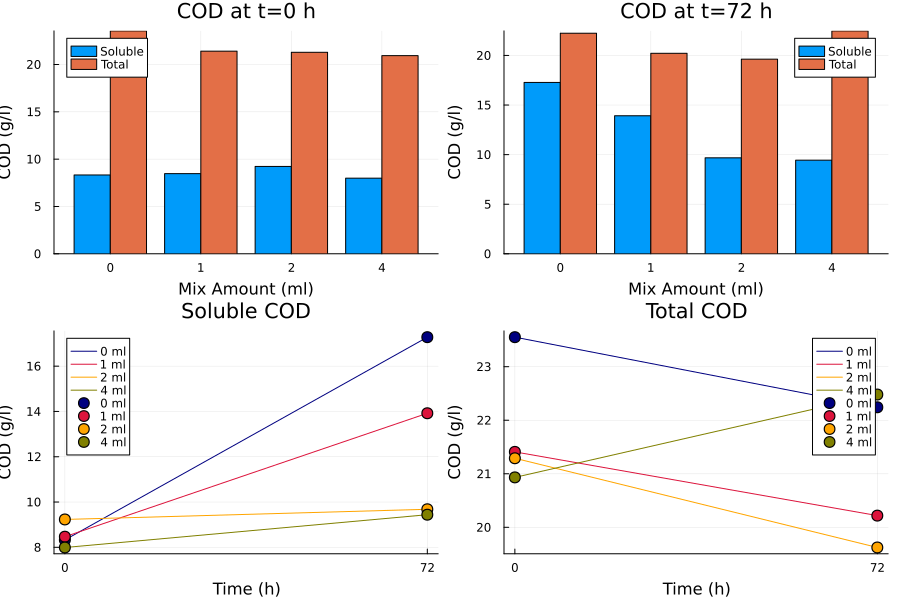
\includegraphics[width=.9\linewidth]{../plots/26_03/complete_cod_plot_26_03.png}
\end{center}

\section{Μετρήσεις στερεών}
\label{sec:org98dd245}
Εκτός από τις παραπάνω αναλύσεις που έγιναν για την μέτρηση του COD των υδρολυμάτων που τροφοδοτηθούν, μία άλλη σημαντική μέτρηση ήταν αυτή των TS και VS των υδρολυμάτων αλλά και της λάσπης. Οι υπολογισμοί που χρειάστηκαν εδώ ήταν πολύ απλοί οπότε δεν χρειάζεται να γίνει data loading σε Julia, καθώς ένα απλό org table μας δίνει όλη την πληροφορία που χρειαζόμαστε. Προζυγίστηκαν οι 4 κάψες και σε αυτές μετρήθηκαν TS και VS των τεσσάρων υδρολυμάτων (0, 1, 2 και 4 ml). Παρακάτω φαίνονται τα αποτελέσματα.

\begin{table}[htbp]
\caption{Μετρήσεις TS και VS για τα food waste}
\centering
\begin{tabular}{rrrrrrrr}
Αριθμός & m\textsubscript{Κάψας} (g) & m\textsubscript{FW} (g) & Ζύγισμα TS (g) & TS & Ζύγισμα VS (g) & VS & VS/TS\\[0pt]
\hline
1 & 14.9116 & 5.4618 & 15.0150 & 18.931488 & 14.9218 & 17.063972 & 0.901\\[0pt]
2 & 15.5253 & 5.2913 & 15.6072 & 15.478238 & 15.5253 & 15.478238 & 1.000\\[0pt]
3 & 15.0313 & 5.7813 & 15.1098 & 13.578261 & 15.0415 & 11.813952 & 0.870\\[0pt]
4 & 11.3655 & 5.7184 & 11.4764 & 19.393537 & 11.3968 & 13.919978 & 0.718\\[0pt]
\end{tabular}
\end{table}

Θα γίνουν όμως imported σε julia για να γίνουν κάποια plots.

\begin{minted}[breaklines=true,breakanywhere=true]{julia}

ts_vs_data = CSV.read(datadir("exp_pro", "hydrolysate_ts_vs_26_03.csv"), DataFrame)
ts = ts_vs_data.TS
vs = ts_vs_data.VS

date = "26_03"
ts_vs_plot = groupedbar(1:4, [vs ts], xticks = (1:4, ["0", "1", "2", "4"]), xlabel = "Mix Amount (ml)", ylabel = "Solids (g/l)", label = ["Volatile" "Total"], title = "Solids Measurements for Hydrolysates")
savefig(ts_vs_plot, get_plot_name("ts_vs", date, "bar_plot"))
\end{minted}

\begin{center}
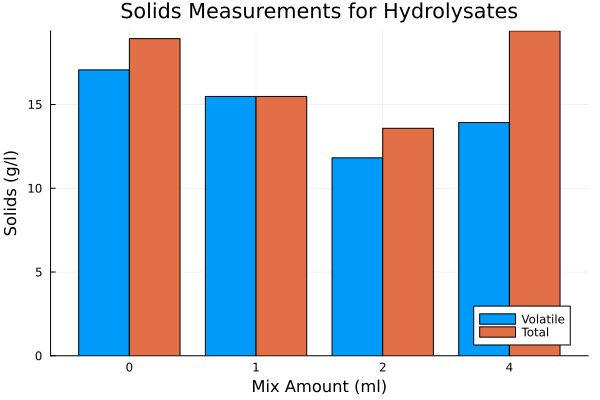
\includegraphics[width=.9\linewidth]{../plots/26_03/ts_vs_bar_plot_26_03.png}
\end{center}

Αντίστοιχη ανάλυση έγινε και για την λάσπη, όπου χρησιμοποιήθηκαν 2 ίδια δείγματα για reproducibility.

\begin{table}[htbp]
\caption{Μετρήσεις TS και VS για την λάσπη}
\centering
\begin{tabular}{rrrrrrrrr}
Αριθμός & Κάψα (g) & m\textsubscript{sl} (g) & v\textsubscript{sl} (ml) & Ζύγισμα TS (g) & TS (g/l) & Ζύγισμα VS (g) & VS (g/l) & VS/TS\\[0pt]
\hline
5 & 14.5440 & 5.7926 & 5.4958254 & 14.8122 & 46.300452 & 14.7419 & 34.164279 & 0.738\\[0pt]
6 & 18.6062 & 8.6804 & 8.2356736 & 19.0077 & 46.253629 & 18.8984 & 33.662043 & 0.728\\[0pt]
\end{tabular}
\end{table}

Από τα αποτελέσματα αυτά υπολογίστηκε πόση λάσπη πρέπει να τροφοδοτηθεί στον αντιδραστήρα για να γίνει η χώνευση που θέλουμε.
\end{document}
